\section{Project Name:} ASSIST (Assistive Smart Stick for Independent and Safe Travel)
 
\section{Introduction: }
Visually impaired go through many hardships when it comes to daily routine tasks, navigation and social life. Plenty are visually impaired around the globe, where many of them are blind and few suffer from partial or color blindness. This concept is devised to supply smart electronic aid that facilitates the impaired with an efficient navigation, obstacle detection and give them artificial sense of vision .

\section{Motivation:}

A person is not disabled,the surrounding and the technology is. We can transfer this disability through technological innovation.Technology can ease life of humans if used in the right direction and a mission in sight. So by using Raspberry Pi and other simple sensors we propose to build a stick that could perform more than just a stick for visually impaired.

\section{Market Research/Literature Survey:}
In 2011, Mr S.Gangwar formulated a smart cane for blind which can give early warning of a hurdle using (IR) sensors. Benjamin Etal in 2011 developed a similar product using laser sensors to determine hurdles and down curbs. The reviewed articles do not provide improvements and enhancements in the places visited by the disabled, stakeholders were limited, analysis and emergency contact feature is absent.

\section{Hardware Requirements:}
\subsection{Raspberry 3B}
Raspberry Pi 3 Model B has a 1.2 GHz 64-bit quad core processor, on-board 802.11n Wi-Fi, Bluetooth and USB boot capabilities.

\subsection{Ultrasonic sensor}
Ultrasonic sensor is a type of sensor that detects an object using sound waves. Its principle is similar to that of radar or sonar, which generates high-frequency sound waves and receives it back.

\subsection{Pi camera}
The Raspberry Pi Camera v2 is a high quality 8 megapixel Sony IMX219 image sensor custom designed add-on board for Raspberry Pi, featuring a fixed focus lens. It's capable of 3280 x 2464 pixel static images, and also supports 1080p30, 720p60 and 640x480p60/90 video. It is used in this smart blind stick for capturing images that are used for object identification. 

\subsection{Vibration motor}
Vibration motor is a compact size coreless DC motor used to informs the users of receiving the signal by vibrating, no sound. The feedback of the obstacle will be provided with a vibration motor.

\subsection{GPS module}
A GPS navigation device, GPS receiver, or simply GPS is a device that is capable of receiving information from GPS satellites and then to calculate the device's geographical position.The application will be designed using a Google Map API, which will provide outdoor navigation as well as provides user location so that the emergency contacts of the user can obtain the location.

\subsection{Gyroscope and Compass}
To determine the orientation of the stick and the angle to turn the direction in.

\section{Software Requirements:}
\subsection
{Python/Django}To create the web portal and represent the data that will be received.

\subsection
{OpenCV/Tensorflow} To process images and to filter the invisible infrastructural design.

\subsection
{Google Maps API} To represent the received location on the map
ChartJS: To represent data in graphical format that will be easy to understand.



\section{Implementation :}
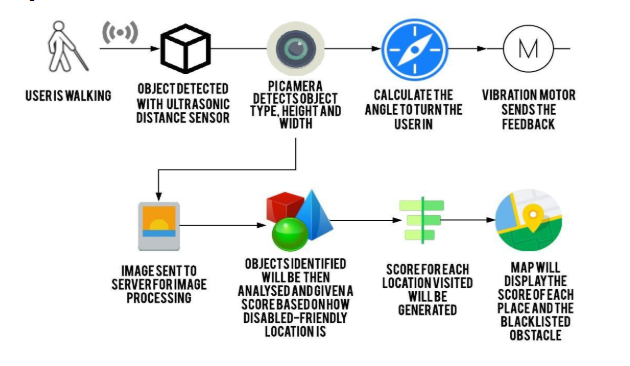
\includegraphics[width=13cm]{implementation}

\begin{itemize}
\item
The user will be walking with the stick embedded with the various sensors and the control kernel
\item
The obstacle will be detected by the ultrasonic sensor which will record the distance and depending on the distance, the presence of an obstacle will be determined.
\item
On detection of an obstacle based on the distance the intensity of the vibration will be changing.
\item
On encountering an obstacle, the Pi camera will click the picture of the obstacle which will be sent to the server for image processing.
\item
The GPS will then relay the location of the person and with the Maps Geocoding API we can obtain the place name from the coordinates sent by the GPS to determine accessibility of the place. 
\item
The dataset of the image processing algorithms will contain images of the types of obstacles that are difficult to traverse through by a differently abled person.
\item
With this dataset and image processing, we can indicate if the place is accessible to everyone.
\item
Each place will be assigned a score based on an algorithm. Accessible and inaccessible places will be displayed on the map along with the flaws in design at these places.
\item
At the same time based on the orientation of the stick, the angle that the user will need to turn in will be determined. By fixing a fixed rotation direction (clockwise or anticlockwise) and the direction of the stick, the user will turn in the given angle to avoid the obstacle. 
\item
The most frequently accessed locations will be also determined and each of these places will be suggested changes depending on the feasibility score.
\item
Suggested changes will include the necessary design changes to be taken care of in the place so as to make it more accessible.
\item
The authorities can view this information and suggested changes and determine the necessary actions to be taken in these places. 
\item
The routes taken by a person is also displayed on the map so as to increment the facilities available in these routes.
\item
In emergency situations, the user on click of a button can notify the emergency contact of their location and thus can have a prompt response.
\end{itemize}


\section{Feasibility:}
\begin{itemize}
   \item Navigation, object detection and orientation are very important factors for ensuring safety and independence of the visually impaired.
   
   \item There are some devices which has become a revolution over the last few decades to guide a visually impaired person and to make their life even easier and safer but these are costly and heavy and most of them doesn’t contain camera and GPS module for providing object detection and location of person for safety.

   \item
   Our system which will be cost effective, reliable, low power consumption solution for navigation with obvious short response time. Ultrasonic sensor and vibration motor will lead to good results in detecting the obstacles on the path and GPS module is useful for providing emergency contacts by tracking user location.
   
   \item Image processing will provide  the images of the obstacle or live stream using pi camera. As many places aren’t disabled friendly, so image processing can help to analyse the difficult designations and hence blacklisting them. 

   \item These infrastructural improvements can be suggested to the government and private agencies in order to make places easily accessible for the differently abled.
\end{itemize}

\section{References:}

\begin{itemize}

\item [1] “Smart walking stick - an electronic approach to assist visually disabled persons”, Mohammad Hazzaz Mahmud, Rana Saha, Sayemul Islam. 

\item [2] “A Multidimensional Walking Aid for Visually Impaired Using Ultrasonic Sensors Network with Voice Guidance”, Olakanmi O. Oladayo Electrical and Electronic Engineering, Technology Drive, Office 6, New Faculty of Engineering Building, University of Ibadan, Ibadan, Nigeria.

\item [3] “Ultrasonic smart cane indicating a safe free path to blind people”, arun G. Gaikwad 1, H. K. Waghmare2 1ME Embedded system Design, MIT Aurangabad ,2 Assistant Professor Department of EXTC, MIT Aurangabad.

\item [4] “Blind navigation system for visually impaired using windowing-based mean on Microsoft Kinect camera” in 2017 Fourth International Conference on Advances in Biomedical Engineering (ICABME).

\item [5] “Mobile phone based indoor navigation system for blind and visually impaired people: VUK — Visionless supporting framework” in 2018 19th International Carpathian Control Conference (ICCC).

\item [6] “Virtual-Blind-Road Following-Based Wearable Navigation Device for Blind People” in IEEE Transactions on Consumer Electronics (Volume: 64 , Issue: 1 , Feb. 2018 ).

\item  [7] ”An Intelligent Walking Stick for the Blind”, Kher Chaitrali S., Dabhade Yogita A., Kadam Snehal K.,Dhamdhere Swati D., Deshpande Aarti V. JSPM’s Jayawantrao Sawant College of Engineering. [10] ”Smart Stick for Blind Man”, Nitish Sukhija1, Shruti Taksali2, Mohit Jain3 and Rahul Kumawat4 1, 3 Student JECRC UDML COLLEGE of Engineering.aired.” 

\end{itemize}



